% Systems programming summary
% written during my studies at ETH Zuerich
% based on the lecture of Prof. Gustavo Alonso and Prof. Thomas Gross 
% Copyright (C) 2004  Patrick Pletscher

\documentclass[german, 10pt, a4paper, twocolumn]{scrartcl}

\usepackage{babel}
\usepackage{amsmath}
\usepackage{amsfonts}
\usepackage[pageanchor=false,colorlinks=true,urlcolor=black,hyperindex=false]{hyperref}
\usepackage[bf]{caption2}
\usepackage{multirow}

\usepackage{pstricks}

\usepackage[dvips]{graphicx}


% text below figures
\renewcommand{\captionfont}{\small\itshape}

% theorems, definitions
\newtheorem{definition}{Definition}

% dimensions of document
\textwidth = 19 cm
\textheight = 25 cm
\oddsidemargin = -1.5 cm
\evensidemargin = -1.5 cm
\hoffset = 0.0 cm
\marginparwidth = 0.0 cm
\topmargin = -1.0 cm
\headheight = 0.0 cm
\headsep = 0.0 cm
\parskip = 0 cm
\parindent = 0.0 cm

% depth of toc
\setcounter{secnumdepth}{2}
\setcounter{tocdepth}{2}

% informations about the document
\title{Systemprogrammierung - Zusammenfassung}
\author{Patrick Pletscher}

\begin{document}

\maketitle

\section{Computerarchitektur}

\subsection{Ressourcen und Operationen}

\subsubsection{Register}

Schnellste Speicherzellen, nur sehr wenige (8-32), beschr"ankte Gr"osse, viele Operationen. K"onnen normalerweise 32 Bit speichern.

\subsubsection{Speicher$[$zellen$]$ (aka Memory)}

Viele Zellen, aber meistens langsam. Die meisten Speicherzellen k"onnen 8 Bit speichern.

\subsubsection{Speichereinheiten}

Speichereinheiten enthalten Bits. Um sich den Inhalt besser vorstellen zu k"onnen, verwandelt man sie ins Hexadezimalsystem.

\subsubsection{Operations}

Die Operationen interpretieren den Inhalt der Speichereinheiten. Eine Speichereinheit kann z.B. Integers, Floats, Characters oder andere Typen enthalten. Die Operationen entscheiden wie man diese Werte benutzt.

\subsection{Core Architektur}

Das Memory ist "uber Bus(es) mit der Computation Unit verbunden, welche wiederum "uber Bus(es) mit den Registern verbunden ist.

\subsubsection{Prozessor (oder CPU - central processing unit)}

Enth"alt die Computation engine (= ALU - arithmetic and logical unit), die Register, das Memory interface und andere spezielle Register.

\subsubsection{Instruktionen}

Eine Operation kontrolliert die Ausf"uhrung einer Operation auf diesem Prozessor. Die Instruktion spezifiziert den Opcode (welche Operation? z.B. \verb#add mul, load, mov#) und welches die Operanden sind. Diese Operationen sind nat"urlich auch bin"ar. Um nicht bin"ar programmieren zu m"ussen gibt es Assemblersprachen.

\subsubsection{Assemblerinstruktionen}

Assembler bieten meisten mehr Funktionalit"at als nur "Ubersetzung, z.B. symbolische Namensaufl"osung und das Definieren von Datensegmentnen (\verb# A: .byte 32#).

\subsubsection{Instruktionsspeicherung}

Auf dem SPARC haben alle Instruktionen die selben Gr"osse von 32 Bit. Die Instruktionen sind im Memory gespeichert.

\subsubsection{Instruktionssequenzierung}

Grundlegende Abfolge:
\begin{itemize}
	\item Hole eine Instruktion
	\item Dekodiere sie
	\item Lese die Operanden
	\item F"uhre die Operation aus
	\item Speichere die Resultate
\end{itemize}

Daf"ur wird eine Ressource ben"otigt, die die Adresse der aktuellen Instruktion speichert: Der PC (=program counter) welcher als Teil der ''Grundlegenden Abfolge'' inkrementiert wird.\\

Wir brauchen auch Instruktionen um den PC zu modifizieren (z.B. f"ur If-then-else) sogenannte \textit{Kontrollflussinstruktionen}.

\subsubsection{Arbeiten mit Adressen}

Wir brauchen symbolische Namen um Adressen mit einer symbolischen Adresse zu versehen. Dabei hilft der Assembler.

\subsubsection{Zusammenfassung}

Drei Arten von Instruktionen:
\begin{itemize}
	\item Berechnungen - z.B. \verb#add, sub, mul, or, xor#
	\item Datenbewegung - z.B. \verb#load, store#
	\item Kontrollfluss - z.B. \verb#goto, jump, branch, call,#\\
		\verb#return#
\end{itemize}

\subsection{Wie werden Programme ausgef"uhrt}

Unterteilung in ''trusted code'' (das Betriebssystem) und ''untrusted code'' (die Anwenderprogramme). Verschiedene Prozesse f"uhren entweder OS oder Anwenderprogramme aus.

\subsubsection{Ausf"uhren des Programmes}

\begin{itemize}
	\item Zu einer bestimmten Zeit entscheidet das OS ein Programm auszuf"uhren.
	\item Ein Prozess nimmt die Instruktionen, reserviert/ erstellt Platz (f"ur Daten) und f"uhrt eine Instruktion nach der anderen aus. Dieses Programm ''besitzt'' nun die CPU.
	\item Diese Aktivit"at endet wenn
		\begin{itemize}
			\item die letzte Instruktion dieses Programmes zum OS zur"uckkehrt (\verb#return#).
			\item das Programm eine illegale Operation ausf"uhrt.
			\item ein Hardwareproblem detektiert wird.
			\item das OS die CPU zur"uck m"ochte.
		\end{itemize}
\end{itemize}

\section{C Programmierung}

\subsection{"Uberblick}

\subsubsection{C Kompilierungs Modell}

\begin{figure}[hbt]
 \begin{center}
 	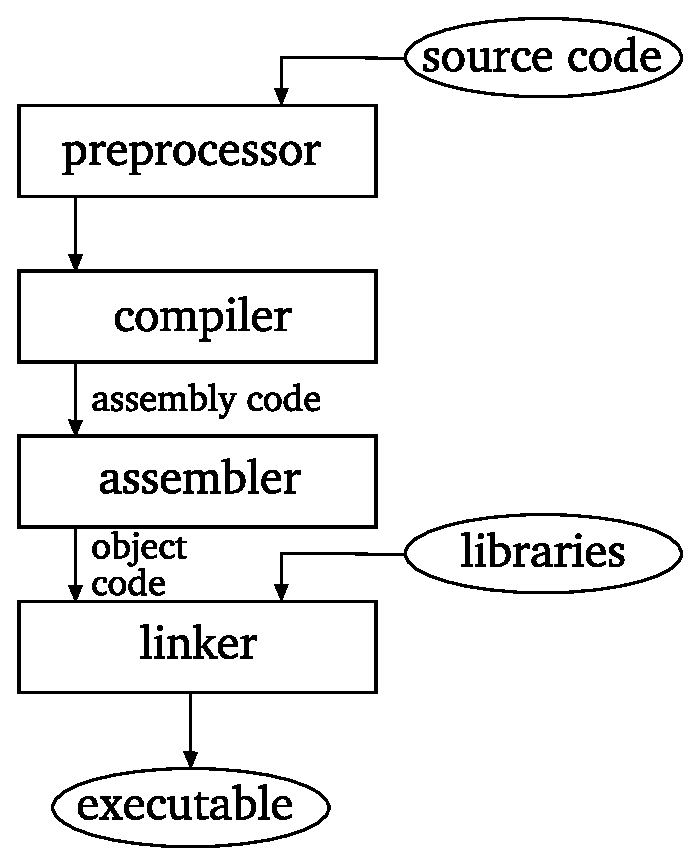
\includegraphics[width=0.4\textwidth]{c_compilation.eps}
 \end{center}
 \label{c_compilation}
 \caption{Ablauf der C Kompilierung}
\end{figure}

\subsubsection{Struktur einen C Programms}

Ein C Programm enth"alt die folgenden Elemente:
\begin{itemize}
	\item Preprocessor Kommandos
	\item Typendefinitionen
	\item Funktionsprototypen (Deklaration von Funktionstypen und -argumenten)
	\item Variablen
	\item Funktionen
\end{itemize}

\begin{verbatim}
 #include <stdio.h>
 #define TIMES 10
 
 double myfunction(float);

 int main(void) {
  double wert;
  double pi = 3.14;
  printf("Multiply by 10\n");

  wert = myfunction(pi);

  printf("%d * %f = %f\n",
          TIMES, pi, wert);
 }

 double myfunction(double zahl){
  double count = 0;

  count = TIMES * zahl;

  return count;
 }
\end{verbatim}

Alle Programme m"ussen eine einzige \verb#main()# Funktion enthalten. Alle Funktionen (auch \verb#main()#) haben folgendes Format:
\begin{verbatim}
 type function_name (parameters){
        local variables
        C Statements
 }
\end{verbatim}

\subsubsection{Datentypen}

C besitzt die folgenden grundlegenden Datentypen\\\\
\tiny
\begin{tabular}{|l|c|c|c|l|}
 \hline
 C Type &		Size (bytes) &		Lower bound &	Upper bound &	Use \\ \hline\hline
 char &			1 &			- &		- &		characters\\ \hline
 unsigned char &	1 &			0 &		255 &		small numbers\\ \hline
 short int &		2 &			-32768 &	+32767 &	integers \\ \hline
 unsigned short int &	2 &			0 &		65536 &		positive int \\ \hline
 (long) int &		4 &			$-2^{31}$ &	$-2^{31}-1$ &	large int \\ \hline
 float &		4 &			$-3.2\cdotp10^{\pm 38}$ &	$+3.2\cdotp10^{\pm 38}$ &	real numbers \\ \hline
 double &		8 &			$-1.7\cdotp10^{\pm 308}$ &	$+1.7\cdotp10^{\pm 308}$ &	large reals \\ \hline
 void &			0 &			- &		- &		no return value \\ \hline
\end{tabular}
\normalsize

\begin{itemize}
	\item Die Gr"osse der Datentypen ist nicht standardisiert, kommt auf die Implementation an.
	\item Der Typ \verb#void# wird f"ur Funktionen benutzt, die keinen Wert oder einen Null-Pointer zur"uckliefern.
	\item Mit \verb@#define@, kann man symbolische Konstanten einf"uhren (z.B. \verb@#define LIMIT 10@).
\end{itemize}

\subsection{Sprachkonstrukte}

\subsubsection{Variablen und Konstanten}

Spezielle Konstanten f"ur die Benutzung mit Strings sind:
\begin{itemize}
	\item \verb#\n# Neue Linie
	\item \verb#\t# Tabulator
	\item \verb#\r# Wagenr"ucklauf (carriage return)
	\item \verb#\b# Backspace
	\item \verb#\"# Escape double quote
	\item \verb#\0# end string
\end{itemize}

\verb#sizeof()# ist eine Funktion die die Gr"osse einer gegebenen Variable in Bytes zur"uckliefert.\\

Variablen sollten vor der Ben"utzung initialisiert werden, da sie sonst einen zuf"alligen Wert enthalten.

\subsubsection{Typenumwandlung (casts)}

Die Umwandlung kann explizit durch den Programmierer geschehen:
\begin{verbatim}
 var_new_type = (new_type) var_old_type

 // Example
 int a;
 float x = (float) a;
\end{verbatim}

Die Umwandlung kann aber auch implizit durch den Compiler geschehen:
\begin{itemize}
 \item \verb#char# und \verb#short# k"onnen zu \verb#int# konvertiert werden
 \item \verb#float# kann zu \verb#double# konvertiert werden
 \item in einem Ausdruck, wenn ein Argument \verb#double# ist, werden alle anderen zu \verb#double# gecastet.
 \item in einem Ausdruck, wenn ein Argument \verb#long# ist, werden alle anderen zu \verb#long# gecastet.
 \item in einem Ausdruck, wenn ein Argument \verb#unsigned# ist, werden alle anderen zu \verb#unsigned# gecastet.
\end{itemize}

\begin{verbatim}
 int a = 3;
 float b = 5.0;
 float c = a + b; // a wird in float umgewandelt
\end{verbatim}

\subsubsection{Scope}

\begin{itemize}
	\item Globale Variablen werden normalerweise vor der main Funktion deklariert, sie sind "uberall sichtbar, sollten aber vermieden werden.
	\item Lokale Variablen sind g"ultig und sichtbar in einem einzigen Block (ein Block ist eine Menge von C Statements umgeben von geschweiften Klammern \{\}). Wenn der Kontrollfluss ausserhalb eines Blockes ist, so existiert die Variable nicht mehr l"anger.
	\item Lokale Variablen werden erstellt (Platz im Memory wird alloziert) wenn der Kontrollfluss den Block erreicht in dem sie deklariert sind und zerst"ort (dealloziert) wenn der Kontrollfluss den Block verl"asst.
	\item Das Erstellen und Zerst"oren von Variablen kann kontrolliert werden:
		\begin{itemize}
			\item \verb#extern#: Die Variable ist in einem anderen Modul definiert
			\item \verb#static#: F"ur lokale Variablen: Bleiben f"ur das ganze Programm; f"ur globale Variablen: beschr"ankt den Scope auf das aktuelle Modul
			\item \verb#register#: Versuche ein CPU Register f"ur die Variable zu benutzen.
			\item \verb#auto#: Vorgabe f"ur lokale Variablen.
		\end{itemize}
\end{itemize}

\subsubsection{Arithmetische Ausdr"ucke}

Die Priorit"at der Operatoren ist mathematisch korrekt.

\begin{verbatim}
 // Addition
 x = 3 + 4;
 // Subtraktion
 x = 10 - 3;
 // Multiplikation
 x = 3 * 4;
 // Division
 x = 3 / 4;
  /* x = 9, if int x */
 x = 73.0 /8.0;
  /* x=9.125, if float x */
 // Modulo
 x = 73 % 8;
\end{verbatim}

\subsubsection{Short-hand Operatoren}

\begin{itemize}
	\item Wenn \verb#++# oder \verb#--# als Prefix verwendet wird, so wird die Variable ver"andert, bevor sie f"ur die Auswertung des Ausdruckes benutzt wird.
		\begin{verbatim}
		 a = 3;
		 b = ++a + 3;
		 /* b = 4 + 3 = 7 und a = 4 Seiteneffekt */
		\end{verbatim}
	\item Wenn \verb#++# oder \verb#--# als Postfix verwendet wird, so wird die Variable zuerst f"ur die Auswertung des Ausdruckes benutzt und wird danach ver"andert.
		\begin{verbatim}
		 a = 3;
		 b = a++ + 3;
		 /* b = 3 + 3 = 6 und a = 4 Seiteneffekt */
		\end{verbatim}
	\item Beinahe alle Operatoren k"onnen mit \verb#=# kombiniert werden
		\begin{verbatim}
		 a += b;  /* a = a + b */
		 a *= b;  /* a = a * b */
		\end{verbatim}
\end{itemize}

\subsubsection{Bit Operatoren}

Die Bit-Operatoren \verb#&# (AND), \verb#^# (XOR) und \verb#|# (OR) ver"andern die Bits nach der Standard Zwei-Werte Logik.

\begin{itemize}
	\item Mit \verb#&# kann man Bits auf $0$ setzen. \verb#a &= 0x00#
	\item Mit \verb#^# kann man Bits umkehren. \verb#a ^= 0xFF#
	\item Mit \verb#|# kann man Bits auf $1$ setzen. \verb#a |= 0xFF#
\end{itemize}

Die Beispiele f"ur \verb#&# und \verb#|# machen nat"urlich eigentlich keinen Sinn.

\subsubsection{Shift Operatoren}

\begin{itemize}
	\item \verb#<<# und \verb#>># werden benutzt um die Position von Bits in einem Byte oder Word zu manipulieren.
	\item Mit \verb#a>>b# werden die Bits in Variable a um b Positionen nach rechts verschoben (die neuen Bits werden mit $0$ gef"ullt).
	\item Mit \verb#a<<b# werden die Bits in Variable a um b Positionen nach links verschoben (die neuen Bits werden mit $0$ gef"ullt).
\end{itemize}

\subsubsection{Vergleich und logische Operatoren}

Die Vergleichsoperatoren liefern $1$ oder $0$ abh"angig vom Resultat des Vergleiches.
\begin{itemize}
	\item \verb#<# kleiner als
	\item \verb#># gr"osser als
	\item \verb#<=# kleinergleich als
	\item \verb#>=# gr"ossergleich als
	\item \verb#==# gleich wie
	\item \verb#!=# nicht gleich wie
\end{itemize}

\verb#&&# und \verb#||# sind die logischen AND und OR Operatoren
\begin{verbatim}
 (a != b) && (c > d)
 (a < b) || (c > d)
\end{verbatim}

\subsubsection{If Anweisung}

\begin{verbatim}
 if (expression)
   statement

 if (expression)
   statement-if
 else
   statement-else
\end{verbatim}

\subsubsection{Switch Anweisung}

\begin{verbatim}
 switch (selector) {
   case int_value1: statement1; break;
   case int_value2: statement2; break;
   case int_value3: statement3; break;
   default: statement4;
 }
\end{verbatim}

Falls \verb#break# nach einem Statement weggelassen wird, so wird danach das n"achste case ausgef"uhrt.\\

Switch kann auch f"ur \verb#char# benutzt werden, da das ja eigentlich auch ein Integer ist.

\subsubsection{for Anweisung}

\begin{verbatim}
 for(initialization; termination; increment) {
   statement
 }
\end{verbatim}

\begin{itemize}
	\item Alle Elemente in der for Schleife sind optinal: \verb#for(;;);#
	\item \verb#break# kann benutzt werden um die Schleife zu beenden, ohne darauf zu warten, dass die terminierende Bedingung zu true ausgewertet wird.
	\item \verb#continue# kann benutzt werden um die Ausf"uhrung des Inhalts der Schleife zu "uberspringen und die terminierende Bedingung neu zu "uberpr"ufen.
\end{itemize}

\subsubsection{while Anweisung}

\begin{verbatim}
 while(expression){
   statement
 }
\end{verbatim}

\verb#break# und \verb#continue# k"onnen wie bei der for Schleife benutzt werden.

\subsubsection{Do-while Anweisung}

Die Do-while Schleife ist "ahnlich wie die while Schleife, ausser dass die Schleife immer einmal durchlaufen wird und dass die Bedingung am Ende jeder Iteration "uberpr"uft wird.

\begin{verbatim}
 do {
   statement
 } while (expression)
\end{verbatim}

\verb#break# und \verb#continue# k"onnen wie bei der for Schleife benutzt werden.

\subsubsection{Ungerade Enden}

\verb#exit()# beendet die Ausf"uhrung des Programmes und "ubergibt dem OS einen Integer Fehlercode. Dabei steht z.B. $0$ f"ur keinen Fehler, $99$ f"ur crash.

\subsection{Arrays}

Die Nummerierung f"ur die Elemente beginnt immer bei $0$. Wenn das Array $N$ Elemente besitzt, so ist das ist das letzte Element an Position $N-1$. Achtung: Der C-Compiler "uberpr"uft die Array-Grenzen nicht.

\begin{verbatim}
 // Variablendeklaration
 int data[5];
 
 // Variablendeklaration mit Initialisierung
 int data[5] = {1,2,3,4,5};

 // Zugriff auf Elemente
 data[3] = 32;
\end{verbatim}

\subsubsection{Mehrdimensionale Arrays}

\begin{verbatim}
 int a[2][2];

 /* im Memory
 +-+-+-+-+-+-+-+-+-+-+-+-+-+-+-+-+-+-+-+-+
 | a[0][0] | a[0][1] | a[1][0] | a[1][1] |
 +-+-+-+-+-+-+-+-+-+-+-+-+-+-+-+-+-+-+-+-+
 */
\end{verbatim}

\subsubsection{Arrays und Strings}

Strings sind Arrays von Buchstaben, terminiert durch den Null Buchstaben \verb#'\0'#.

\begin{verbatim}
 char str[6] = {'h','a','l','l','o','\0'};
 char str[6] = "hallo";
\end{verbatim}

\subsubsection{Arrays und Pointers}

Arrays und Pointers sind f"ur den Compiler dasselbe. Der Array-Name ist ein Pointer zum Anfang des Arrays.

\subsection{Pointers}

Eine Variable hat einen Namen, eine Adresse, einen Typ und einen Wert:
\begin{itemize}
	\item Der Name identifiziert die Variable f"ur den Programmierer
	\item Die Adresse gibt an, wo im Hauptspeicher die Variable zu finden ist, d.h. dem Anfang des Speicherbereichs der f"ur die Variable reserviert wurde.
	\item Der Typ gibt an, wie man die Daten im Speicher zu interpretieren hat und wie gross die Variable ist.
	\item Der Wert ergibt sich aus den aktuellen Daten der Variablen interpretiert nach dem Typ.
\end{itemize}

Pointers sind Sprachkonstrukte, die es dem Programmierer erlauben die Adresse von Variablen direkt zu manipulieren.

\begin{verbatim}
 int* px;  /* px = pointer to an integer */
 
 int x;

 px = &x;  /* px bekommt die Adresse von x */

 x = *px;  /* x bekommt den Inhalt davon */
           /* worauf px zeigt */

 /* Der Nullpointer wird so definiert */
 int* n_ptr = NULL;
\end{verbatim}

Um einem Addressbereich der in einem Pointer \verb#int* nummer_ptr# gespeichert z.B. einen Wert zuzuweisen benutzt man:
\begin{verbatim}
 *nummer_ptr = 7;
\end{verbatim}

Mehrere Pointer aufeinander:
\begin{verbatim}
 int* *p_ptr_ptr;
 p_ptr_ptr = &nummer_ptr;
 /* p_ptr_ptr zeigt nun auf den Speicherbereich
    von nummer_ptr dort ist wiederum ein 
    anderer Speicherbereich gespeichert wo dann
    ein wirklicher Wert steht
 */

 *(*p_ptr_ptr) = 5;
\end{verbatim}

\subsubsection{Pointers, Arrays und Strings}

Ein Array is in Wirklichkeit ein Pointer:
\begin{verbatim}
 int a[10],y;
 int* px;
 px = a;     /* px points to a[0] */
 px++;       /* px points to a[1] */
 px = &a[4]; /* px points to a[4] */

 px = a;
 y = *(px+3); /* y gets the value */
              /* in a[3] */
\end{verbatim}

Die Pointerarithmetik von C garantiert, dass wenn ein Pointer inkrementiert oder dekrementiert wird, er gem"ass seinem Typ ver"andert wird. Zum Beispiel, falls \verb#px# auf ein Array zeigt, so wird \verb#px++# immer zum n"achsten Element zeigen, unabh"angig was der Typ des Arrays ist.

\subsection{Structures}

Structures erlauben es dem Programmierer komplexe Datentypen zu definieren.

\begin{verbatim}
 struct Id_card {
   char name[100];
   char address[100];
   short int geburtsjahr;
   int telefon;
   short int semester;
 } ethz, uniz;
\end{verbatim}

Structures vom selben Typ k"onnen mit dem Operator \verb#=# kopiert werden, sollten aber nicht mit \verb#==# verglichen werden.\\

Um Zugriff auf die Elemente eines struct zu erhalten, geht man wie folgt vor:
\begin{verbatim}
 ethz.name = "Hans Muster";
 ethz.telefon = 1234;
\end{verbatim}

Pointers k"onnen auch auf structs zeigen, man kann darauf mit \verb#-># oder \verb#*# zugreifen.
\begin{verbatim}
 struct Id_card *pid;
 pid = &ethz_student;
 pid->name = "Hans Muster";
 /* oder aber */
 (*pid).name = "Hans Muster";
\end{verbatim}

\subsection{Funktionen}

\begin{verbatim}
 returntype function_name(def of parameters) {
   localvariables
   functioncode
 }
\end{verbatim}

\subsubsection{main() ist auch eine Funktion}

F"ur das Einlesen von Kommandozeilenargumenten kann man wie folgt vorgehen:
\begin{verbatim}
 int main(int argc, char **argv){
   code
 }
\end{verbatim}

\begin{itemize}
	\item \verb#argc# enth"alt die Anzahl "ubergebener Argumente.
	\item \verb#argv# Array der "ubergebenen Argumente.
	\item \verb#argc# ist immer mindestens $1$, da \verb#argv[0]# der Programmname ist.
\end{itemize}

\subsection{Dynamic Memory allocation}

Die Funktionen f"ur Memoryallozierung sind in \verb#stdlib.h# zu finden. Typische Funktionen sind \verb#malloc# und \verb#free#.

\begin{verbatim}
 typedef struct node {
   int x,z;
   struct node *next;
 } NODE;

 NODE *nptr;
 if ((nptr = ((NODE)*)malloc(sizeof(NODE)))
  == NULL) {
   printf("No memory - bye bye"); exit(99);
 }
\end{verbatim}

\verb#malloc# gibt einen Pointer zum allozierten Memory zur"uck. Der Pointer ist generisch (\verb#void *#), darum ist es eine gute Idee den Pointer zum gew"unschten Typ zu casten um Fehler zu vermeiden.

\subsection{String library}

\begin{verbatim}
 #include <stdio.h>
 #include <string.h>

 void main() {
   char name1[12], name2[12], mixed[25];
   char title[20];

   strcpy(name1, "Rosalinda");
   strcpy(name2, "Zeke");
   strcpy(title, "This is the title");

   printf("  %s\n\n", title);
   printf("Name 1 is %s\n", name1);
   printf("Name 2 is %s\n", name2);

   if (strcmp(name1,name2) > 0)
     /* returns 1 if name1 > name 2*/
     strcpy(mixed, name1);
   else
     strcpy(mixed, name2);


   printf("The biggest name alphabetically is
    %s\n", mixed);

   strcpy(mixed, name1);
   strcpy(mixed, " ");
   strcpy(mixed, name2);
   printf("Both names are %s\n", mixed);
 }

 /*
 
 will generate:

   This is the title
 
 Name1 is Rosalinda
 Name2 is Zeke
 The biggest name alphabetically is Zeke
 Both names are Rosalinda Zeke
 
 */
\end{verbatim}

\section{Computer Arithmetik und Informationsspeicherung}

\subsection{Umwandlung dezimal - bin"ar}

Um eine Zahl von dezimal $d$ nach bin"ar $b$ umzuwandeln geht man wie folgt vor:
\begin{enumerate}
	\item b := ''''
	\item Finde $k$ so dass $2^{k+1}> d \geq 2^{k}$.
	\item Dividiere $d$ ganzzahlig durch $2^k$ und h"ange die resultierende $1$ oder $0$ hinten an $b$ heran.
	\item Setze $d$ gleich dem Rest der Division.
	\item Setze $k=k-1$ und falls $k \geq 0$ gehe zu 2.
\end{enumerate}

\subsection{Darstellung von Buchstaben}

ASCII character set stellt Buchstaben mit 7 Bits dar, urspr"unglich keine Unterst"utzung f"ur spezielle Symbole wie z.B. "u. Heute im Normalfall 8 Bits. In Assembler k"onnen Buchstaben wie folgt benutzt werden:
\begin{verbatim}
 mov   0140, %r1  ! as octal
 mov   'a', %r1
 mov   "a", %r1
\end{verbatim}

\subsection{Darstellung von Integer}

\begin{itemize}
	\item \textit{unsigned}: Jedes Bit wird mit positivem Gewicht interpretiert.
	\item \textit{two's complement f"ur signed}: Erstes Bit negatives Gewicht, der Rest mit positivem Gewicht.
	\item binary to unsigned
		\begin{displaymath}
			b2u(x_{n-1},\ldots,x_0) = \sum^{n-1}_{i = 0} x_i\cdotp 2^i
		\end{displaymath}
	\item binary to two's complement
		\begin{displaymath}
			b2t(x_{n-1},\ldots,x_0) = -x_{n-1} + \sum^{n-2}_{i = 0} x_i\cdotp 2^i
		\end{displaymath}
	\item Es treten nat"urlich Probleme auf, wenn man eine unsigned Zahl als signed interpretiert.
\end{itemize}

C spezifiziert keine Darstellung f"ur signed, die meisten Computer benutzen two's complement. Signed ist die Vorgabe \verb# int x; /* signed */#.

\subsection{Modulus Arithmetik}

Computer benutzen of Modulus Arithmetik. Modulus Arithmetik ber"ucksichtigt nur Zahlen in einem Bereich $[0,M)$. Falls wir in der Modulus Arithmetik die gr"osste m"ogliche Nummer $M-1$ erreichen, gehen wir rundherum und starten wieder bei $0$.\\

Wenn wir eine Operation von zwei Zahlen ausf"uhren und das Resultat "uberschreitet den Modulus, so sagen wir ein \textit{Overflow} sei aufgetreten.

\subsubsection{Complement's}

Complement's sind wichtig, da man eine Subtraktion in eine Addition umwandeln kann.
\begin{displaymath}
	a-b = a + (r^n -1 -b)+1
\end{displaymath}
Dabei ist $r^n-1-b+1$ das Radixkomplement f"ur Zahlen mit $n$ Ziffern, welch eine System mit Basis $r$ benutzen.\\

F"ur bin"are Nummern kann man das two's complement ganz einfach finden, in dem man alle Bits umkehrt und 1 dazu addiert.

\subsubsection{Status flags}

F"ur signed:
\begin{itemize}
	\item N (negativ) bit: Gesetzt falls MSB 1 ist.
	\item Z (zero) bit: Gesetzt falls alle Bits 0 sind.
	\item V (overflow) bit: Gesetzt falls 
		\begin{itemize}
			\item in $c=a-b$ $a$ und $b$ unterschiedliche Vorzeichen haben und $c$ und $b$ die gleichen haben.
			\item in $c=a+b$ $a$ und $b$ das gleiche Vorzeichen haben, aber unterschiedlich von $c$.
		\end{itemize}
\end{itemize}

F"ur unsigned: Overflow wird durch ein C (carry) bit detektiert, welches gesetzt wird, wenn "Ubertrag vom MSB auftritt. Bei der Subtraktion hingegen ist dieses Bit gesetzt falls das Resultat positiv ist und sonst $0$.\\
C Bit wird gesetzt, falls Carry auftritt bei MSB bei Addition und wenn es nicht auftritt bei Subtraktion, also wenn Carry-Bit nicht gesetzt bei Subtraktion, so ist das Resultat positiv.

\section{SPARC Assembler}

\subsection{"Ubersicht}

\subsubsection{Struktur eines Assembler Programmes}

Assembler Programme sind linienorientiert. Der Assembler unterscheidet 4 verschiedene Typen von Linien:
\begin{itemize}
	\item leere Linie
	\item Labeldefinitions Linie. Ein Identifier gefolgt von einem Kolon ('':'').
	\item Direktiven Linie. Eine optionale Labeldefinition gefolgt von einer Assemblerdirektive, gefolgt von den Argumenten der Direktive.
	\item Instruktions Linie. Eine optionale Labeldefinition gefolgt von einem Operatornamen, gefolgt von den Operanden.
\end{itemize}

\subsubsection{Segmente und Anweisungen}

Ein Assembler Programm enth"alt drei Segmente:
\begin{itemize}
	\item data: Konstanten und Platz f"ur Daten.
	\item text: Die Instruktionen.
	\item BSS (Block Storage Segment): Platz f"ur dynamische Daten (aka ''heap'') und nicht initialisierte globale Variablen.
\end{itemize}

Eine Anweisung:
\begin{verbatim}
 label: instruction
 ! instruction ist eine Maschineninstruktion
 ! oder eine synthetische Operation

 label: directive
\end{verbatim}

In Assembler kann man mit verschiedenen Systemen arbeiten:
\begin{itemize}
	\item Hexadezimal \verb#0x...#
	\item Oktal \verb#0...#
	\item Dezimal
\end{itemize}

\subsubsection{Beispiel}

\begin{verbatim}
         .data
 a:      .word 0x11
 
         .text
 start:  ta 0
\end{verbatim}

\subsubsection{SPARC Register}

SPARC ist ein "load/store architecture". Also nur die load und store Anweisungen greifen auf das Memory zu, alle anderen Operanden m"ussen in Registern sein.\\

SPARC hat 32 Integer Register (jedes Register enth"alt 32 Bit), die \verb#%r0 ... %r31# benannt sind.\\

Es gibt aber auch alternative Namen:
\begin{itemize}
	\item Globale Register (\verb#%g0 ... %g7#) -- \verb#%r0 ... %r7#
	\item Ausgabe Register (\verb#%o0 ... %o7#) -- \verb#%r8 ... %r15#
	\item Lokale Register (\verb#%l0 ... %l7#) -- \verb#%r16 ... %r23#
	\item Eingabe Register (\verb#%i0 ... %i7#) -- \verb#%r24 ... %r31#
\end{itemize}

Spezielle Register:
\begin{itemize}
	\item \verb#%g0# (\verb#%r0#) ist immer \verb#0x0#.
	\item \verb#%o6# (\verb#%sp,%r14#) ist der Stackpointer.
	\item \verb#%o7# (\verb#%r15#) ist die R"ucksprungadresse von der aufgerufenen Subroutine.
	\item \verb#%i6# (\verb#%fp,%r30#) ist der Framepointer.
	\item \verb#%i7# (\verb#%r31#) ist die Subroutine R"ucksprungadresse.
\end{itemize}


\subsubsection{Direktiven}

\begin{itemize}
	\item \verb#.ascii string1, ..., stringn#\\
		z.Bsp.: \verb#.ascii "Hello world\n"#
	\item \verb#.global# Macht ein Label global
	\item \verb#.byte val1, ..., valn#\\
		z.Bsp.: \verb#.byte 0xf1#
	\item \verb#.word val1, ..., valn#
	\item \verb#.halfword val1, ..., valn#
	\item \verb#.include "filename"#
\end{itemize}

\subsection{Grundlegende Instruktionen}

\subsubsection{Programanfang}

Der Anfang eines Programmes wird durch die Direktive \verb#.text# angezeigt.

\begin{verbatim}
 .text
 start: ...
\end{verbatim}

\subsubsection{Programmende}

Die Ausf"uhrung sollte man mit der Instruktion \verb#ta# beenden. Dies ist eine Trapinstruktion die das OS aufruft mit einer Aufforderung ins Register \verb#%g1#.

\begin{verbatim}
 end:  ta 0
\end{verbatim}

\subsubsection{set}

Laden von Konstanten in ein Register.

\begin{verbatim}
 set  0x42, %r2
 set  x, %r3
\end{verbatim}

\subsubsection{clear}

Die \verb#clr# Operation setzt einen bestimmten Speicherbereich auf 0. Diese Operation ist synthetisch.

\begin{verbatim}
 clr  [%r3]
 clr  a  /* a declared in .data segment */
\end{verbatim}

\subsubsection{load}

Holt ein word aus dem Memory in ein Register.

\begin{verbatim}
 ld  [%r2], %r3
\end{verbatim}

\subsubsection{store}

Kopiert den Wert eines Registers (word) in den Speicher.

\begin{verbatim}
 st  %r3, [%r2]
\end{verbatim}

\subsubsection{move}

Kopiert den Inhalt eines Registers oder eine kleine Konstante in ein anderes Register. Diese Instruktion ist synthetisch.

\begin{verbatim}
 mov  %r1, %r2
 mov  1, %r2
\end{verbatim}

\subsubsection{add, sub}

Brauchen drei Argumente: zwei Operanden und als drittes Argument das Zielregister f"ur das Resultat. Die Operanden k"onnen entweder 2 Register sein oder ein Register und eine signed small constant (13 bit).

\begin{verbatim}
 add %r3, %r4, %r5  ! %r5 = %r3 + %r4
 sub %r3, 1, %r3    ! %r3 = %r3 - 1
\end{verbatim}

\subsubsection{signed und unsigned Multiplikation}

Multiplikation von zwei 32-bit Werten, welche ein 64-bit Resultat liefern. Die most significant 32-bit werden im \verb#%y# Register gespeichert und die restlichen 32-bit im Zielregister. Das zweite Argument kann eine kleine Konstante sein.

\begin{verbatim}
 smul  %r1, %r2, %r3
 umul  %r1, 10, %r3
\end{verbatim}

\subsubsection{null Operation}

Die \verb#nop# Operation "uberspringt einen Zyklus, in dem sie nichts tut.

\begin{verbatim}
 nop
\end{verbatim}

\subsubsection{signed und unsigned Division}

Die Ganzzahldivision teilt ein 64-bit Wert durch ein 32-bit Wert und speichert das Resultat im Zielregister. Das \verb#%y# Register enth"alt die most significant 32-bit und das erste Register die restlichen 32-bit.

\begin{verbatim}
 sdiv  %r1, %r2, %3  ! %r3 = {%y,%r1}/%r2
 udiv  %r1, 10, %3   ! %r3 = {%y,%r1}/10
\end{verbatim}

\subsection{Instruktionspipelining}

In einer Pipeline Architektur, wird jede Instruktion in verschiedene Teile aufgeteilt und seperat ausgef"uhrt. Diese Teile sind: Fetch, Decode, Operand fetch, Execute, Store. Zu jedem Zeitpunkt werden gleichzeitig mehrere Instruktionen ausgef"uhrt. 2 Instruktionen, die ausgef"uhrt werden sind sichtbar: \verb#%pc, %npc#.

\subsubsection{Probleme mit Pipelines}

Hazard: Wenn es einem Instruktionsstadium in der Pipeline unm"oglich ist etwas w"ahrend des Zyklus auszuf"uhren. Hazards k"onnen in mehreren Situationen auftreten:
\begin{itemize}
	\item Datenabh"angigkeiten: Ben"otigte Daten sind noch nicht bereit.
	\item geteilte Ressourcen: Die Funktionseinheit die ben"otigt wird, wird im Moment benutzt.
	\item control branches: Wir wissen nicht welche Instruktion als n"achstes ausgef"uhrt wird.
\end{itemize}

\subsubsection{Branching hazards}

Die Pipeline wird automatisch mit der n"achsten Instruktion gef"ullt, welche sowieso ausgef"uhrt wird (\verb#%pc,%npc#). Aber wenn wir springen, ist die Instruktion die ausgef"uhrt wurde ung"ultig. Die einfachste L"osung daf"ur ist es nach der branch Instruktion ein \verb#nop# einzuf"ugen.\\
Der branch delay slot kann benutzt werden um eine Instruktion auszuf"uhren.

\subsection{Branching in Assembler}

Spezielles condition code (cc) Register, mit dem man bestimmte Charakteristiken des Resultats einer bestimmten Anweisung testen kann. Dieses spezielle Register hat 4 bits:
\begin{itemize}
	\item Z (Zero): 1 wenn Resultat 0 war.
	\item N (Negative): 1 wenn Resultat negativ war.
	\item C (Carry): carry bit des MSB vom Resultat
	\item V (oVerflow): Zeigt an, dass ein Resultat zu gross war um in ein Register zu passen.
\end{itemize}

Nicht alle Operationen setzen diese Bits, spezielle Operationen werden ben"otigt:
\begin{verbatim}
 addcc, subcc
 smulcc, sdivcc
\end{verbatim}

Im Folgenden ist Target ein label. Der Branch wird nur gemacht, wenn die Bedingung true ist, sonst geht die Ausf"uhrung nach der branch Instruktion weiter.\\

\scriptsize
\begin{tabular}{lll}
	Operation &		Assembler syntax &	Branch condition \\ \hline
	Branch always &		\verb#ba    target# &	1 (always)\\
	Branch never &		\verb#bn    target# &     0 (never)\\
	Branch not equal &	\verb#bne   target# &	not Z\\
	Branch equal &		\verb#be    target# &     Z\\
	Branch greater &	\verb#bg    target# &     not(Z or(N xor V))\\
	Branch less or equal &	\verb#ble   target# &    Z or (N xor V)\\
	Branch greater or equal &		\verb#bge   target# &     not(N xor V)\\
	Branch less &		\verb#bl    target# &     N xor V\\
	Branch greater, unsigned &		\verb#bgu   target# &     not (C or Z)\\
	Branch less or equal, unsigned &		\verb#bleu  target# &     C or Z\\
	Branch carry clear &	\verb#bcc   target# &     not C\\
	Branch carry set &	\verb#bcs   target# &     C\\
	Branch positive &	\verb#bpos  target# &     not N\\
	Branch negeative &	\verb#bneg  target# &     N\\
	Branch overflow clear &	\verb#bvc   target# &     not V\\
	Branch overflow set &	\verb#bvs   target# &     V\\
\end{tabular}
\normalsize

\subsection{While Schleife}

Bedingungen k"onnen mit \verb#cmp# gepr"uft werden. Dies ist eine synthetische Instruktion, und wird durch eine Subtraktion mit "Ubertrag bewerkstelligt.

\begin{verbatim}
  cmp  register1, register2
  cmp  register2, const.
\end{verbatim}

Die folgende while Schlaufe in C:
\begin{verbatim}
 main() {
   int a = 0;
   int b = 3;
   while (a <= 17) {
     a = a + b;
   }
 }
\end{verbatim}

Kann in Assembler z.Bsp. so ausssehen:
\begin{verbatim}
          .data
 a:       .word 8
 b:       .word 3
          .global _main
	  
          .text
 _main:   set     a, %r1
          ld      [%r1], %r2
          set     b, %r1
          ld      [%r1], %r3

 loop:    cmp     %r3, 17
          ble, a  loop
          add     %r2, %r3, %r2

  store:  set     a, %r1
          st      %r2, [%r1]

  end:    ta      0
\end{verbatim}

\verb#ble, a# ist dabei ein sogenannter annuled branch delay slot, diese Instruktion wird also ausgef"uhrt, falls gesprungen wird und sonst nicht.

\subsubsection{Annuled Branches}

Die Anweisung nach einem annuled branch wird als annuliert markiert, falls der Branch nicht gemacht wird und dann wird mit der Instruktion in \verb#%npc# fortgefahren. 

\subsection{do while Schlaufen}

Gleich wie while Schlaufe, nur dass dort vor dem Loop noch einmal alle Instruktionen im Loop ausgef"uhrt werden.

\subsection{If-then else}

\begin{verbatim}
 if ((a+b) >= c) {
   a += b;
   c++;
 else {
   a -= b;
   c--;
 }
 c += 10;
\end{verbatim}


\begin{verbatim}
              ! a -> %r2, b -> %r3, c -> %r4
              add    %r2, %r3, %r6
              cmp    %r6, %r4
              bl,a   else             ! if
              sub    %r2, %r3, %r2    ! 1. in else
              add    %r2, %r3, %r2    ! 1. in if
              inc    %r4
              ba     store
              add    %r4, 10, %r4
 else:        dec    %r4
              add    %r4, 10, %r4
 store:       set    a, %r1
              st     %r2, [%r1]
 end:         ta     0
\end{verbatim}

\subsection{switch}

\begin{verbatim}
 switch(i) {
   case 1:   i += 1;
             break;
   case 2:   i += 2;
             break;
   case 15:  i += 15;
   case 3:   i += 3;
             break;
   case 4:   i += 4;
   case 6:   i += 6;
             break;
   case 5:   i += 5;
             break;
   default   i--;
 }
\end{verbatim}


\small
\begin{verbatim}
            .data
            .align  4
 table:     .word   L1,L2,L3,L4,L5,L6,L7,L8,L9
            .word   L10,L11,L12,L13,L14,L15

            .text
            .align  4
 start:     set     i, %r1
            ld      [%r1], %l0
            ld      [%r1], %o0    ! %o0 = i
            cmp     %o0, 1
            blu     default       ! too small
            cmp     %o0, 15       ! too large
            nop
            set     table, %o1    ! jump table
            sll     %o0, 2, %o0   ! %o0 x 4
            add     %o1, %o0, %o0
                     ! %o0 points to case in
                     ! table
            jmpl    %o0, %g0
            nop
 L1:        ba      end
            add     %l0,1,%l0     ! i++
 L2:        ba      end
            add     %l0,2,%l0     ! i+=2
 L15:       add     %l0,15,%l0    !i+=15, no break
 L3:        ba      end
            add     %l0,3,%l0     !i+=3
 L4:        add     %l0,4,%l0     !i+=4, no break
 L6:        ba      end
            add     %l0,6,%l0     !i+=6
 L5:        ba      end
            add     %l0,5,%l0     !i+=5
 L7:
 L8:
 L9:
 L10:
 L11:
 L12:
 L13:
 L14:
 default:   sub     %l0,1,%l0     !i--
 end:       ta      0
\end{verbatim}
\normalsize

\section{Caching}

\subsection{Cache Architekturen}

\begin{description}
	\item[Direct-mapped cache]: Die Memoryadresse bestimmt eindeutig die zugeh"orige Cache Linie.
	\item[Fully associative]: Eine Memoryadresse kann irgendwo im Cache gespeichert werden. Es gibt keine im Konflikt stehenden Adressen. Sehr teuer, da man den ganzen Cache durchsuchen muss um eine Memoryadresse zu finden.
	\item[Set associative cache]: Cache Linien unterteilt in Mengen, Memoryadressen zeigen auf die Mengen (mittlere Bits, nicht die untersten Bits). In einer Menge ist die Zuweisung v"ollig assoziativ. Zwei Memoryadressen stehen im Konflikt, wenn sie auf die gleiche Menge zeigen. Aber in der gleichen Menge gibt es verschiedene Positionen wo die Adressen hin k"onnen. Typische Mengengr"ossen sind 4.
\end{description}


\section{Arithmetische Operationen in Assembler}

\subsection{Boolsche Operationen}

F"ur Boolsche Ausdrucke gibt es folgende Ausdr"ucke:
\begin{verbatim}
 ! Benutzung wie folgt:
 !b_op    r1, r2, dest_reg

 and      r1 AND r2
 andn     r1 AND ~r2
 or       r1 OR r2
 xor      r1 XOR r2
 xnor     r1 XOR ~r2
 orn      r1 OR ~r2
\end{verbatim}

NOT kann wie folgt bewerkstelligt werden:
\begin{verbatim}
 not      source_reg, dest_reg
 xnor     source_reg, %g0, dest_reg
\end{verbatim}

\subsection{Test Operationen}

\begin{verbatim}
 ! a -> %l1
 ! Verschiedene Moeglichkeiten fuer das 
 ! Testen nach a > 0
 
 cmp     %l1, 0
 ble     next
 
 ! cmp ist synthetisch und wird
 ! uebersetzt zu

 subcc   %l1, %g0, %g0
 ble     next
 
 ! Alternativ kann man auch tst benutzen
 
 tst     %l1
 ble     next

 ! tst ist synthetisch und wird
 ! uebersetzt zu

 orcc    %l1, %g0, %g0
\end{verbatim}


\subsection{Addition von Bin"arzahlen}

Die Summe zweier Zahlen in bin"ar Darstellung ist gleich einer XOR-Verkn"upfung und der "Ubertrag kann mit einem AND berechnet werden.

\begin{verbatim}
 add (int a, int b) {
   
   sum = a^b;
   
   while (carry = (a&b) << 1){
     a = sum;
     b = carry;
     sum = a^b;
   }

   return(sum);
 }
\end{verbatim}

\subsection{Multiplikation von Bin"arzahlen}

\begin{displaymath}
 \underbrace{23}_{\mbox{Multiplicand}}\times \underbrace{32}_{\mbox{Multiplier}}
\end{displaymath}

Grobe Abfolge (genaueres siehe Abbildungen im Skript):
\begin{enumerate}
	\item Falls hinterstes Bit von Muliplier 0 so kopiere 0 zu Temp, sonst kopiere Multiplicand nach Temp.
	\item Addition von Temp und bisherigem Produkt nach Produkt.
	\item $\{ Produkt,Multiplier \}$ um 1 nach rechts shiften.
	\item Gehe wieder zu 1 falls noch nicht ganz Multiplier durchgeshiftet, mit jetztigen Werten in Produkt und Multiplier.
\end{enumerate}

Bei der unsigned Multiplikation wird am Ende das two's complement vom Multiplicand gebildet und dann wie folgt vorgegangen:
$\{Produkt,Multiplier \}+\{TWC,0\ldots0 \}$ wobei $TWC$ das two's complement vom Multiplicand ist.

\subsubsection{Division}

siehe Skript

\section{Stack und Datenstrukturen}

\subsection{Memory}

32 Bit SPARC Architektur hat 4 Gigabytes Addressraum.

\subsubsection{Memory aus Sicht von Assembler}

Speicherdatentypen in Assembler sind byte, halfword, word und doubleword (in C meist: char, short, int, long). Manipulation dieser Positionen im Speicher durch load und store. Die Speicheradressen sind nach Standardl"angen aligniert. Die Adressen sind also in der Form $n\cdotp2$ f"ur half-words, $n\cdotp4$ f"ur words und $n\cdotp 8$ f"ur doubles.

\subsection{Stack}

In der SPARC Architektur werden Anwendungsprogramme irgendwo oberhalb von der Position 0x2000 im Speicher geladen. Das Runtime-System stellt zus"atzlichen Speicherbereich f"ur die sogenannten automatischen Variablen (z.Bsp. lokale Variablen einer Funktion) zur Verf"ugung. Dieser Speicherbereich ist im oberen Bereich der Speicheradressen und ist als FILO organisiert $\rightarrow$ Stack. Der Stack dient auch zur Zwischenspeicherung von Variablen die sich bei einem Subroutinen-Aufruf in Registern befinden.\\
Der Stack w"achst im Memory von oben nach unten, die Adresse der letzten benutzen Speicherposition ist im \verb#%sp# (=\verb#%o6#) gespeichert. Der Speicher oberhalb des \verb#%sp# wird benutzt.\\
Der Stackpointer ist immer doubleword aligniert (teilbar durch 8).\\
Zus"atzlicher Speicher auf dem Stack kann alloziert werden indem man den stack pointer zu einer tieferen Position im Speicher verschiebt. Der Platz der so alloziert wird, ist der Platz zwischen vorheriger Position und jetztiger Position.
\begin{verbatim}
 sub %sp, 64, %sp
 ! provides additional 64 bytes of memory on stack.
\end{verbatim}

\subsection{Alignment}

Alignment wird bewerkstelligt in dem man die 3 letzten Bits einer two's complement Bin"arnummer auf 0 setzt.\\

In Assembler wird dies mit einer AND Operation gemacht:
\begin{verbatim}
 add  %sp, -94 & 0xfffffff8, %sp
 ! or
 add  %sp, -94 & -8, %sp ! provides 96 bytes
\end{verbatim}

\subsection{Framepointer}

Typische Subroutinen allozieren automatische Variablen wenn sie aufgeruft werden und darum wird der Stackpointer beim Aufruf der Subroutine erh"oht. Wenn das passiert, dann wird der alte Wert im Framepointer (\verb#%fp# oder \verb#%i6#) gespeichert.\\

Eine spezielle Instruktion wird benutzt um den Stackpointer zu erh"ohen und den alten Wert in den Framepointer zu speichern, dadurch wird Platz f"ur die automatischen Variablen in den Registern und im Hauptspeicher reserviert.
\begin{verbatim}
 save %sp, -64 - bytes_of_local_storage, %sp
 ! 64 bytes for register variables/contents
\end{verbatim}

Beispiel f"ur das Reservieren von 5 Variablen (word size):
\begin{verbatim}
 save %sp, (-64 - (5*4)) & -8, %sp
\end{verbatim}

Der Assembler wertet die arithmetischen Ausdr"ucke aus.

\subsection{Zugriff auf den Stack (load)}

Das Alignment muss ber"ucksichtigt werden. Adressen werden relativ zum Stackpointer \verb#%sp# oder dem Framepointer \verb#%fp# berechnet. Double words werden in ein Paar von Registern geladen oder davon gespeichert.\\

Load Instruktionen sind:\\

\begin{tabular}{lp{6.5cm}}
	\verb#ldsb# &		load signed byte (propagte sign to the left)\\
	\verb#ldub# &		load unsigned byte\\
	\verb#ldsh# &		load signed halfword (propagte sign to the left)\\
	\verb#lduh# &		load unsigned halfword\\
	\verb#ld# &		load word\\
	\verb#ldd# &		load double, register number must be even and the load occurs on register n and n+1
\end{tabular}\\

Eine load Instruktion braucht zwei Zyklen um die Daten vom Memory zu holen. Das System verz"ogert automatisch die Pipeline, wenn die n"achste Instruktion diese Daten ben"otigt.

\subsection{Zugriff auf den Stack (store)}

Store Instruktionen sind:\\
\begin{tabular}{lp{6.5cm}}
	\verb#stb# &		store low byte of register (bits 0-7)\\
	\verb#sth# &		store low two bytes of register\\
	\verb#st# &		store register\\
	\verb#std# &		store double, register number must be even, first four bytes from register n, the other 4 from register n+1
\end{tabular}

\subsection{Lokale Variablen auf dem Stack}

\subsubsection{Variablen Offset und Alignment}

Man benutzt meistens Symbole um die Offset-Konstanten zu definieren.
\begin{verbatim}
 int a,b;
 char ch;
 short c;
 int d;

 ! wird zu:

 a_s = -4
 b_s = -8
 ch_s = -9
 c_s = -12
 d_s = -16

 ! [..]
 ld [%fp + a_s], %l1
\end{verbatim}

Die Offsets m"ussen den Alignment-Vorlagen gen"ugen und sind immer relativ zum \verb#%fp# adressiert, die Offsets f"ur lokale Variablen sind folglich negativ.

\begin{figure}[htb]
	\begin{center}
	\psset{unit=0.4cm,yunit=0.4cm, xunit=0.55cm}
	\begin{pspicture}(-2.5,1)(12,17)

		\psframe(1,1)(5,6.2)
		\psframe[fillcolor=lightgray, fillstyle=solid](1,6.2)(5,7)
		\psframe(1,7)(5,10)
		\psframe(1,10)(5,16)

		\put(-0.6,1.1){\texttt{\%fp}}
		\put(3,3.8){lokale}
		\put(2.1,2.8){Variablen}

		\put(2,8.9){Funktions-}
		\put(2,7.9){parameter}
		\put(-2.5,10.1){\texttt{\%sp} +92}

		\put(2.3,13){Register}

		\put(-0.6,16){\texttt{\%sp}}


		\psline{<-}(6.5,14)(6.5,4)
		\put(10,7){kleiner}


	\end{pspicture}
	\end{center}
	\caption{Position von lokalen Variablen im Stackframe}
\end{figure}

\begin{description}
	\item[lokale Variablen] Werden relativ zum \verb#%fp# adressiert.
	\item[Padding] Zwischen den lokalen Variablen und den Funktionsparametern gibt es m"oglicherweise 4 Bytes Padding, da der \verb#%sp# 8 Bytes aligniert sein muss.
	\item[Funktionsparameter] Immer 4 Byte Bereiche, auch f"ur \verb#short# oder \verb#char#.
\end{description}

%\begin{figure}[hbt]
% \begin{center}
% 	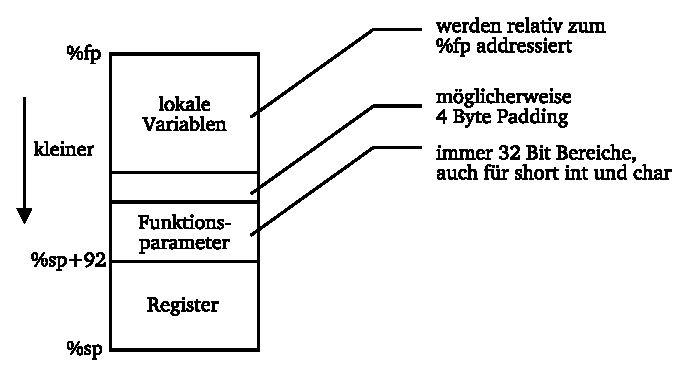
\includegraphics[width=0.4\textwidth]{stack.eps}
% \end{center}
% \label{stack}
% \caption{Position von lokalen Variablen im Stackframe}
%\end{figure}
%
\subsection{Structs}

Structs werden als zusammenh"angender Block gespeichert. Members sind auf ihre Gr"osse aligniert. Das Struct selbst ist auf die Gr"osse des gr"ossten Members aligniert.\\

%\begin{figure}[hbt]
% \begin{center}
% 	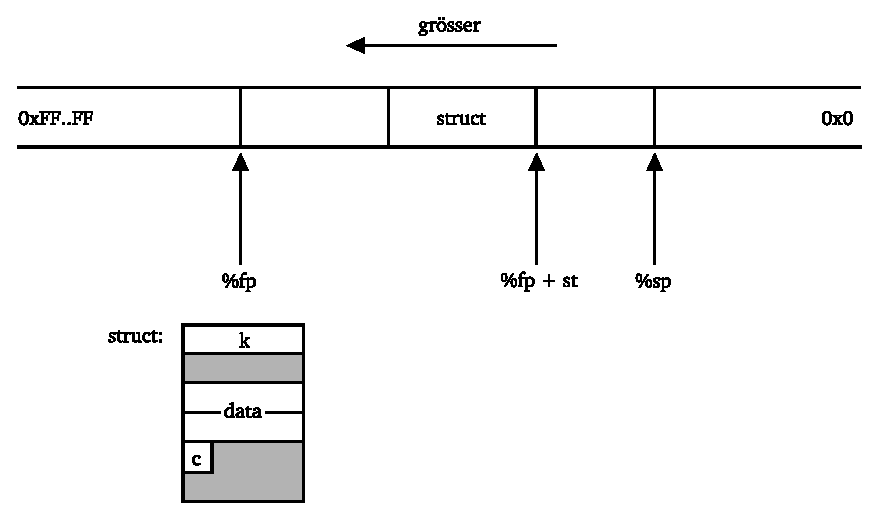
\includegraphics[width=0.4\textwidth]{struct.eps}
% \end{center}
% \label{struct}
% \caption{Struct in Stackframe}
%\end{figure}
%
%\begin{verbatim}
% struct st{
%   int k;
%   double data;
%   char c;
% }
%\end{verbatim}
%
%\begin{verbatim}
% Offsets:
%   st = -40
% 
%   st_k = 0
%   st_data = 8
%   st_c = 16
%\end{verbatim}

Ein Beispiel w"are zum Beispiel folgendes struct.

\begin{verbatim}
 struct FOO {
    int a;
    float b;
    char c;
    double d;
    char i;
    short s;
 }
\end{verbatim}

\begin{figure}[htb]
	\begin{center}
	\psset{unit=0.9cm,yunit=0.9cm, xunit=1cm}
	\begin{pspicture}(-1,1)(6,9)
		%\psgrid[subgriddiv=0,gridlabels=7pt,gridcolor=lightgray, griddots=10](1,1)(5,6)
		\psline[linecolor=lightgray, linestyle=dotted]{-}(2,1)(2,9)
		\psline[linecolor=lightgray, linestyle=dotted]{-}(3,1)(3,9)
		\psline[linecolor=lightgray, linestyle=dotted]{-}(4,1)(4,9)

		\psframe[fillstyle=solid, fillcolor=lightgray](1,1)(5,2)
		\psframe(1,2)(2,3)
		\psframe[fillstyle=solid, fillcolor=lightgray](2,2)(3,3)
		\psframe(3,2)(5,3)
		\psframe(1,3)(5,5)
		\psframe[fillstyle=solid, fillcolor=lightgray](1,5)(5,6)
		\psframe(1,6)(2,7)
		\psframe[fillstyle=solid, fillcolor=lightgray](2,6)(5,7)
		\psframe(1,7)(5,8)
		\psframe(1,8)(5,9)

		\put(0.2,1.3){$28$}
		\put(0.2,2.3){$24$}
		\put(0.2,3.3){$20$}
		\put(0.2,4.3){$16$}
		\put(0.2,5.3){$12$}
		\put(0.2,6.3){$\ 8$}
		\put(0.2,7.3){$\ 4$}
		\put(0.2,8.3){$\ 0$}

		\psline{-}(1,4)(1.5,4)
		\psline{-}(5,4)(4.5,4)

		\put(1.55,2.3){\texttt{e}}
		\put(4.4,2.3){\texttt{f}}
		
		\put(2.85,3.3){\texttt{\%lo(d)}}
		\put(2.85,4.3){\texttt{\%hi(d)}}

		\put(1.55,6.3){\texttt{c}}

		\put(3.2,7.3){\texttt{b}}
		\put(3.2,8.3){\texttt{a}}
	\end{pspicture}
	\end{center}
	\caption{Beispiel eines Structs im Speicher}
\end{figure}

Die Gr"osse des struct ist folglich 40 Byte und sein Alignment 8 Byte. F"ur die Offsets erbigt sich:
\begin{verbatim}
 st = -40

 st_a = 0
 st_b = 4
 st_c = 8
 st_d = 16
 st_e = 24
 st_f = 26
\end{verbatim}
Wobei angenommen wird, dass das struct die erste lokale Variable ist (somit ergibt sich ein \verb#st=-40#).\\

Auf Element \verb#e# kann nun wie folgt zugegriffen werden:
\begin{verbatim}
 ld [%fp + st + st_e], %o0
\end{verbatim}

Structs Offsets sind positive Ganzzahlen, w"ahrend Stackvariablen Offsets negativ sind. Die Structelemente liegen also in umgekehrter Reihenfolge auf dem Stack.\\

\subsubsection{Erl"auterungen}

\begin{enumerate}
	\item Struct wird als zusammenh"angender Block gespeichert.
	\item Elemente sind immer auf ihre Gr"osse aligniert, deshalb ergeben sich teilweise Paddings.
	\item Alignment des Struct ist die Gr"osse seines gr"ossten Members; falls das Struct eine Gr"osse hat, welche modulo seines Alignments ungleich Null ist, so wird am Ende des Struct ein Padding eingef"ugt, so dass es seinen Alignmentvorgaben entspricht.
	\item Bei der "Ubersetzung eines C Programms in Assember werden Elemente in der Reihenfolge des C Codes immer an der kleinst m"oglichen Stelle gespeichert, welche den Alignmentvorgaben entspricht. Es wird aber immer an h"oherer Stelle als das vorhergehende gespeichert.
\end{enumerate}

\subsection{Arrays}

Die Adresse eines Elementes eines Arrays wird durch einen Pointer auf die Basisadresse des Arrays plus ein Offset berechnet. Um in einem Array von words das Element \verb#a[2]# zu laden benutzt man:
\begin{verbatim}
 mov  2, %l0
 sll  %l0, 2, %o0 ! multiply *4
 add  %fp, %o0, %o0
 ld   [%o0 + a_base], %o0
\end{verbatim}

Hier ein Beispiel f"ur ein Integer Array.

\begin{verbatim}
 int array[5];
\end{verbatim}

\begin{figure}[htb]
	\begin{center}
	\psset{unit=0.9cm,yunit=0.9cm, xunit=1cm}
	\begin{pspicture}(-1,1)(6,6)
		%\psgrid[subgriddiv=0,gridlabels=7pt,gridcolor=lightgray, griddots=10](1,1)(5,6)
		\psline[linecolor=lightgray, linestyle=dotted]{-}(2,1)(2,6)
		\psline[linecolor=lightgray, linestyle=dotted]{-}(3,1)(3,6)
		\psline[linecolor=lightgray, linestyle=dotted]{-}(4,1)(4,6)

		\psframe(1,1)(5,2)
		\psframe(1,2)(5,3)
		\psframe(1,3)(5,4)
		\psframe(1,4)(5,5)
		\psframe(1,5)(5,6)

		\put(-0.6,1.3){$\texttt{arr}+16$}
		\put(-0.6,2.3){$\texttt{arr}+12$}
		\put(-0.6,3.3){$\texttt{arr}+8$}
		\put(-0.6,4.3){$\texttt{arr}+4$}
		\put(-0.6,5.3){$\texttt{arr}+0$}

		\put(3,1.3){\texttt{a[4]}}
		\put(3,2.3){\texttt{a[3]}}
		\put(3,3.3){\texttt{a[2]}}
		\put(3,4.3){\texttt{a[1]}}
		\put(3,5.3){\texttt{a[0]}}

	\end{pspicture}
	\end{center}
	\caption{Beispiel eines Arrays im Speicher}
\end{figure}

\section{Subroutinen}

Werden durch jump Instruktionen aufgerufen. Der Inhalt von Registern muss f"ur einen Subroutinen Aufruf auf dem Stack gespeichert werden. Auch die Adresse der Aufrufinstruktion wird gespeichert, sie wird return address genannt. Diese Adresse wird in \verb#%o7# bzw. \verb#%i7# in der Subroutine gespeichert. Aufrufe von Subroutinen sind verz"ogert, daher ist die aktuelle R"ucksprungadresse \verb#%i7+8# (zwei 32bit Instruktionen nach dem Aufruf), hier in Subroutine.

\subsection{Auruf von Subroutinen}

Wenn der Name der Subroutine gegeben ist:
\begin{verbatim}
 call <name>
\end{verbatim}
Speichert den \verb#%pc# in \verb#%o7# und hat einen delay slot.\\

Wenn die Adresse der Subroutine zur Laufzeit berechnet wird, dann wird der Aufruf wiefolgt gemacht:
\begin{verbatim}
 jmpl <source_reg>, <dest_reg>
\end{verbatim}
\verb#jmpl# ruft die Funktion an der Adresse die im Register \verb#<source_reg># gespeichert ist auf. Der \verb#%pc# wird im \verb#<dest_reg># gespeichert. Der return aus einer Subroutine wird auch mit dem jump \& link Mechanismus gemacht:
\begin{verbatim}
 jmpl %i7 + 8, %g0
 ! discards the %pc
\end{verbatim}

Was "aquivalent ist zu:
\begin{verbatim}
 ret
\end{verbatim}

\subsection{Subroutinen und der Stack}

\begin{verbatim}
 save %sp, -64, %sp
\end{verbatim}
\begin{itemize}
	\item Speichert die Register \verb#%l0-%l7#, \verb#%i0-%i7# auf dem Stack (in die zu Verf"ugung stehenden 64 Bytes).
	\item Kopiert die Register \verb#%o0-%o7# nach \verb#%i0-%i7#.
	\item F"uhrt eine Addition aus (meistens daf"ur gebraucht um mehr Platz auf dem Stack zu erhalten).
\end{itemize}

\begin{verbatim}
 restore
\end{verbatim}
\begin{itemize}
	\item Kopiert die Register \verb#%o0-%o7# von \verb#%i0-%i7#.
	\item L"adt den Inhalt von den Registern \verb#%l0-%l7#, \verb#%i0-%i7# vom Stack.
	\item F"uhrt eine Addition aus.
\end{itemize}

\subsection{Typischer Subroutinen Aufruf}

\begin{verbatim}
 main:
 ...
 call mysubr
 nop             ! or something meaningful
 ...
 mysubr:
 save %sp, -112, %sp
 ...
 ret
 restore         ! fills delay slot of ret
\end{verbatim}

\subsection{Argument"ubergabe}

Die SPARC Architektur benutzt die Register \verb#%o0,..,%o5# zur Argument"ubergabe an Subroutinen. Wenn mehr als sechs Argumente ben"otigt werden oder f"ur gr"ossere Datenstrukturen wird der Stack benutzt.

\subsubsection{Stackframe}

Im Stackframe wird gespeichert:
\begin{itemize}
	\item lokale Variablen der Prozedur
	\item "Ubergabeparameter f"ur callee's
	\item Struct pointer f"ur callee's welche structs zur"uckgeben
	\item Register Window
	\item evtl. Padding
\end{itemize}

\onecolumn

\begin{figure}[hbt]
 \begin{center}
 	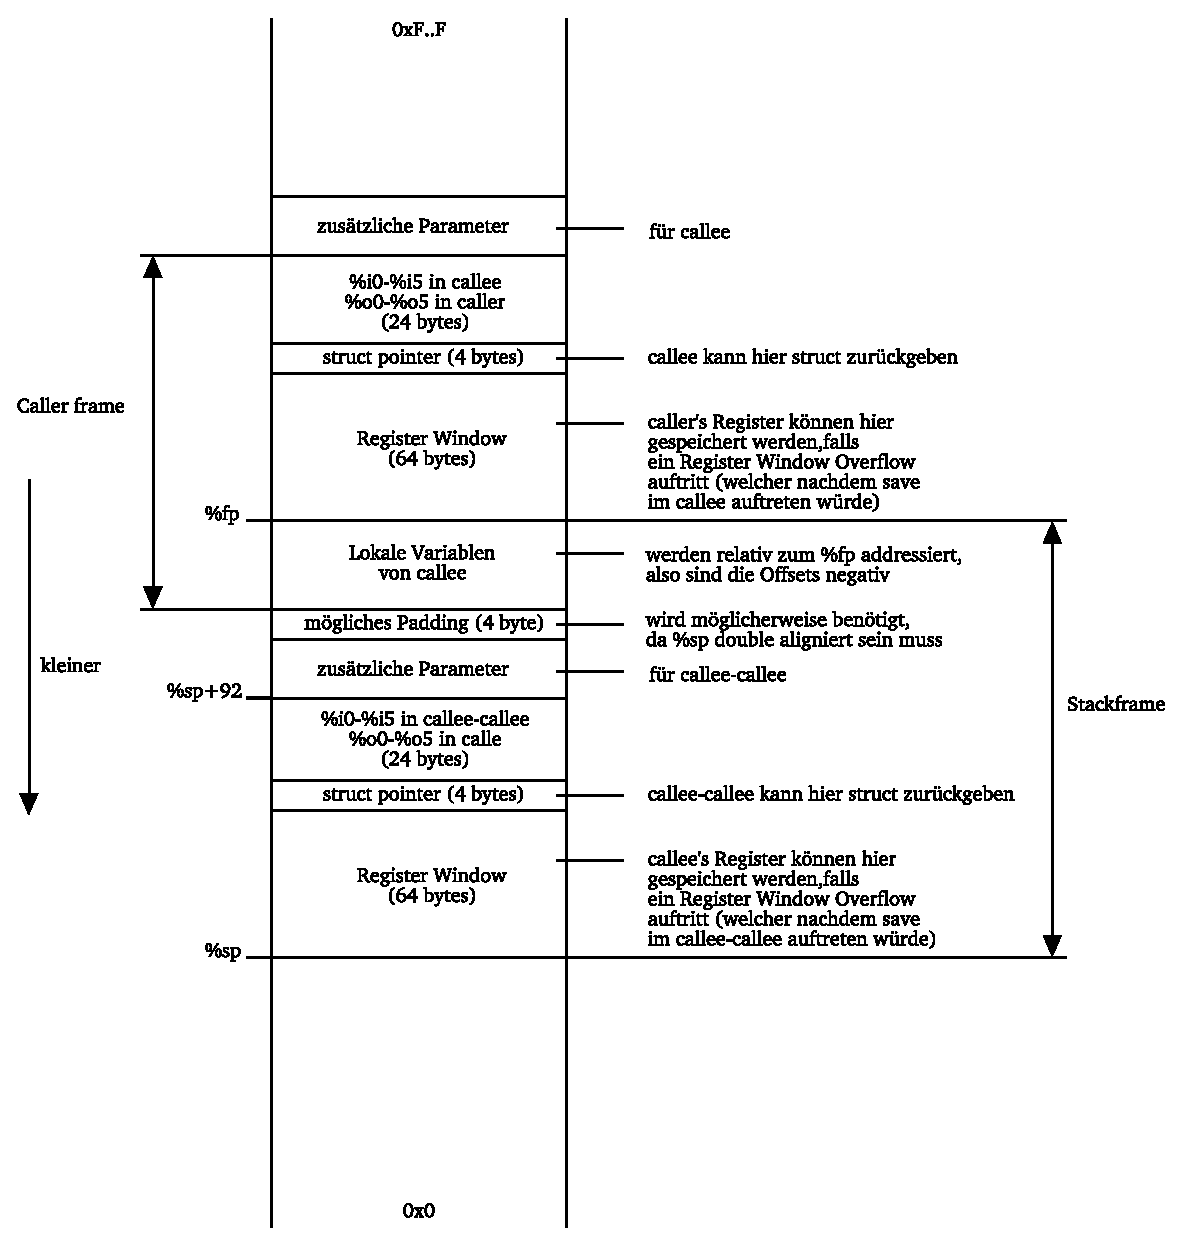
\includegraphics[width=0.9\textwidth]{stackframe.eps}
 \end{center}
 \label{stackframe}
 \caption{Aufbau des Stackframe}
\end{figure}

Es gilt zu beachten, dass Structs by value in lokalen Variablen gespeichert werden und eine Reference darauf "ubergeben wird.

\twocolumn

\subsubsection{Calling Conventions}

\begin{itemize}
	\item Parameter werden in den Registern \verb#%o0-%o5# "ubergeben
	\item Falls Prozedur mehr als 6 Parameter hat, werden diese auf dem Stack (ab Adresse \verb#%sp+92#) "ubergeben, ein Wort pro Parameter und jeweils so, dass sie den oberen Teil des Wortes ausf"ullen.
	\item Spezialf"alle
		\begin{itemize}
			\item structs by value
			\item long long int, double
			\item R"uckgabe von structs
		\end{itemize}
\end{itemize}

\subsubsection{structs by value}

Problem: struct passt evtl. nicht in ein Register. L"osung: Intern werden structs immer by-reference "ubergeben, also mit einem Pointer auf die struct. Wenn also eine Prozedur einen value struct Parameter hat, wird im Stack eine lokale Kopie abgelegt, und ein Pointer auf diese "ubergeben.

\subsubsection{long long int, double}

8 Byte lange Basistypen werden in einen High- und einen Lowteil aufgeteilt, und nacheinander "ubergeben.\\

Beispiel:
\begin{verbatim}
 void foo(long long int x){ .. }
\end{verbatim}

Die hohen 32 Bits von x landen in \verb#%o0#, die tiefen in \verb#%o1#. Auch m"oglich, dass high bits in \verb#%o5#, und low bits an der Adresse \verb#%sp+92# landen, also zur H"alfte in einem Register, zur H"alfte auf dem Stack.

\subsubsection{Beispiel f"ur Stackframe und Parameter"ubergabe}

\begin{verbatim}
 struct s {
   int key;
   long long int data;
   char c;
 }

 void foo(i1,...,i6){
   short k;
   struct s st;
   .
   .
   bar(i1,...,i6,k,&st);
   .
   .
 }
\end{verbatim}

\begin{figure}[hbt]
 \begin{center}
 	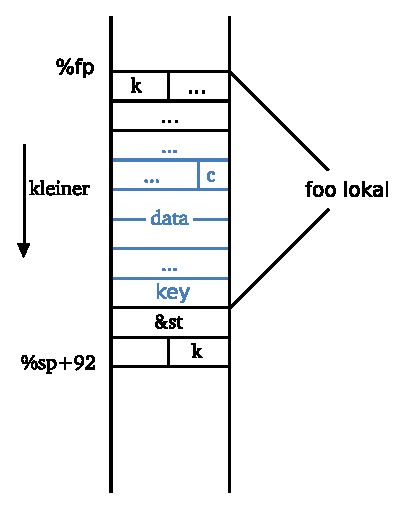
\includegraphics[width=0.4\textwidth]{stack_beispiel.eps}
 \end{center}
 \label{stack_beispiel}
 \caption{Stack nach dem Aufruf von save in bar}
\end{figure}

\subsection{R"uckgabe von Parametern}

Parameter werden in \verb#%o0# zur"uckgegeben, im Callerwindow, also in \verb#%i0# im Calleewindow. Wenn eine Struct zur"uckgegeben werden soll, dann wird der Structure Pointer im Callerframe benutzt, dieser liegt an der Stelle \verb#%fp+64#. Structure Pointer m"ussen vom Caller initialisiert werden, so dass er auf einen g"ultigen Speicherbereich zeigt.

\subsubsection{restore}

Die \verb#restore# Anweisung unterst"utzt wie gesagt eine zus"atzliche Addition, also falls die Summe von zwei Werten in \verb#%o0# bzw. \verb#%o1# (im Callee) zur"uckgegeben werden soll, dann kann man wie folgt vorgehen:
\begin{verbatim}
 restore %o0, %o1, %o0
\end{verbatim}
Zu bemerken ist, dass die Destination \verb#%o0# ist und nicht \verb#%i0#, dies da dies schon wieder im Caller ist.

\subsubsection{unimp}

Falls ein struct zur"uckgegeben werden soll, so legt der Caller als eine weitere Besonderheit nach dem Delayslot eine \verb#unimp# Instruktion an, deren Argument die Gr"osse des f"ur die struct bestimmten Speicherbereichs enth"alt. Also muss der Callee sowohl "uber den Delayslot als auch die \verb#unimp# Instruktion springen.
\begin{verbatim}
 jmpl %i7+12, %g0  ! jump past unimp
\end{verbatim}

\subsection{Leaf Subroutinen}

Leaf-Prozeduren sind Prozeduren welche ...
\begin{itemize}
	\item keine Funktionsaufrufe t"atigen.
	\item kein eigenes Register Window anfordern, also keine \verb#save#/\verb#restore# Instruktionen
	\item Nur auf \verb#%o0-%o5# und \verb#%g1# arbeiten (da sie kein eigenes Window haben).
\end{itemize}

Der R"ucksprung ist anders, da \verb#%pc# in \verb#%o7#, nicht in \verb#%i7#
\begin{verbatim}
 jmpl  %o7+8, %g0
 
 ! oder Synonym fuer obiges
 retl
\end{verbatim}

\section{Register Speicherung und Traps}

Dass nicht jedes Mal wenn eine Subroutine aufgerufen wird, die Register in den Hauptspeicher kopiert werden m"ussen, wird ein Pool von Registern benutzt und ein Fenster (CWP bits im PSR (=processor status register)) das auf die aktuellen Register zeigt. Wenn eine Subroutine eine neue Menge von Registern (in, local, out) ben"otigt so wird einfach der CWP (Current Window Pointer) verschoben:
\begin{itemize}
	\item Die Ausgabe von caller A wird der Input vom callee B.
	\item \verb#%o6# ist der \verb#%sp# von A und wird abgebildet auf \verb#%i6# f"ur B, wo B seinen \verb#%fp# findet.
	\item \verb#%o7# ist die Adresse der aufrufenden Instruktion in A und wird abgebildet auf \verb#%i7#, wo B nach der R"ucksprungadresse sucht, wenn er fertig ist.
	\item \verb#%o0-%o5# sind die "Ubergabeargumente von A an B, B findet sie in \verb#%i0-%i5#.
	\item save: \verb#cwp--#
	\item restore: \verb#cwp++#
\end{itemize}

Somit muss nur der CWP verschoben werden, was sehr schnell gemacht werden kann. Die Additionsoperationen von \verb#save# und \verb#restore# haben eine Besonderheit: das Destinationsregister ist im neuen Set von Registern.
\begin{verbatim}
 save %sp, -64, %sp   ! die zwei %sp sind
                      ! unterschiedlich
\end{verbatim}

\subsection{Register overflow/underflow}

Es gibt nur eine beschr"ankte Anzahl von Registern, in der SPARC Architektur z.B. 7 (also 6 Calls). Was passiert wenn wir sie alle benutzt haben:
\begin{itemize}
 \item Der CWP erreicht den WIM (welcher das Ende der Registersets anzeigt) und ein Hardware Trap tritt ein.
 \item Der Trap resultiert in einem Programm, das aufgerufen wird und die Register auf den Stack kopiert, so dass Platz f"ur Register der aufgerufenen Subroutine entstehen.
 \item Daf"ur wird der Platz verwendet, der vorher mit der \verb#save# Operation reserviert wurde benutzt.
\end{itemize}

\subsection{Register windows}

\texttt{CWP} ist ein Counter
\begin{itemize}
	\item geht herum, "ahnlich Modulus
	\item save: \verb#CWP--#
	\item restore: \verb#CWP++#
\end{itemize}

\texttt{WIM} ist eine Maske von Bits
\begin{itemize}
	\item geht herum, "ahnlich Modulus
	\item Bit geht nach rechts bei einem Overflow. Z.Bsp. 0x08, 0x04, 0x02, 0x01, 0x08, 0x04, 0x02
	\item Bit geht nach links bei einem Underflow. Z.Bsp. 0x01, 0x02, 0x04, 0x08, 0x01, 0x02, 0x04
\end{itemize}

Es hat immer ein Windows "ubrig f"ur Traps.

\subsection{Ablauf eines Overflow Traps}

Es wird versucht einen \verb#save# auszuf"uhren, aber \verb#WIM[--CWP] == 1#, es tritt also ein Overflow auf, somit wird der Overflow trap handler aufgerufen, mit dem Registerset CWP (nach Subtraktion). Der Trap handler geht wiefolgt vor:
\begin{itemize}
	\item \verb#CWP--# (nocheinmal), so dass der \texttt{CWP} jetzt auf dem Registerset ist, das etwas enth"alt, was gespeichert werden muss.
	\item Speichere nun \verb#%lx# und \verb#%ix# in den Speicher an \verb#mem[%sp]#.
	\item Rotiere das \texttt{WIM}, so dass es jetzt auf das aktuelle \texttt{CWP} zeigt.
	\item $\texttt{CWP}+2$
	\item Der \texttt{CWP} ist wieder auf dem urspr"unglichen Registerset, \texttt{CWP--} ist frei und somit hat die \verb#save# Instruktion dieses Mal Erfolg.
\end{itemize}

\subsection{Ablauf eines Underflow Traps}

Es wird versucht ein \verb#restore# auszuf"uhren, aber \verb#WIM[++CWP] == 1#, es tritt also ein Underflow auf, der Trap handler wird gestartet:
\begin{itemize}
	\item $\texttt{CWP}-2 \mod \texttt{NWINDOWS}$
	\item Den \texttt{WIM} rotieren, $\texttt{WIM}[\texttt{CWP}+3 \mod \texttt{NWINDOWS}] = 1$
	\item $\texttt{CWP}+2$
	\item Laden von \verb#%lx,%ix# vom Speicher \verb#mem[%sp]#
	\item Das Register ist jetzt restored
	\item $\texttt{CWP--}$
	\item \texttt{CWP} nun wieder bei urspr"unglichem Registerset vor \verb#restore#
\end{itemize}

\subsection{Trap Maschinerie}

Wenn wir zu einem Traphandler springen, so arbeiten wir manchmal f"ur das Programm, das gerade ausgef"uhrt wird (z.Bsp. Register window overflow) oder wir arbeiten f"ur ein anderes Programm (z.Bsp. Mausbewegungen oder Disk I/O). Die Maschine muss irgendwie zwischen diesen beiden Situationen unterscheiden. Die L"osung ist, dass die Hardware verschiedene Modes unterst"utzt, einen User mode und einen System mode.

\subsection{Definitionen}

Sind nicht standardisiert!

\begin{description}
	\item[Interrupt:] Asynchrone Unterbrechung des Instruktionsfluss. Wird durch ein externes Ereignis verursacht. Kann eine Programmausf"uhrung zwischen 2 Instruktionen treffen.
	\item[Exception:] Unerwartetes Ereignis w"ahrend der Ausf"uhrung des Programmes (Division durch Null, Page fault). Trifft w"ahrend einer Instruktion ein.
	\item[Trap:] Softwaregenerierter Interrupt. Wird durch eine Exception oder durch eine expliziete trap Instruktion (z.Bsp. ein Systemcall) ausgel"ost.
\end{description}

\subsection{Trapinstruktionen txx}

Springe zu OS code um gewisse Funktionen auszuf"uhren. Die Programmausf"uhrung wird vom Usercode zum Systemcode transferiert. Der Zustand der Maschine (CPU) wird gespeichert und wird wiederhergestellt beim Zur"uckkehren zum Usercode (return von Trap: rett). \verb#txx# ist nicht verz"ogert!

\subsection{Status Register des Prozessors}

\begin{description}
	\item[Y-Register:] f"ur Multiplikation und Division: lesen und schreibe mit \verb#rdy,wry# im Usermode.
	\item[PC und nPC:] lesen und schreiben ist implizit durch \verb#jmpl, ret, ...# im Usermode.
	\item[PSR Processor State Register:] lesen und schreiben nur im Superusermodues (\verb#%psr, rdpsr, wrpsr#)
	\item[WIM Window Invalid Mask Register:] lesen und schreiben nur im Superusermodus (\verb#%wim, rdwim, wrwim#).
	\item[TBR Trap Base Register:] lesen und schreiben nur im Superusermodus (\verb#%tbr, rdtbr, wrtbr#)
\end{description}

\subsubsection{Processor State Register (PSR)}

besteht aus verschiedenen Bits, unter anderem:
\begin{itemize}
	\item \texttt{ET}: aktiviere Trap: \texttt{ET == 1}, w"ahrend einem Trap: \texttt{ET == 0}.
	\item \texttt{CWP}
\end{itemize}

\subsubsection{Window Invalid Mask (WIM)}

k Flags um die k Registersets zu implementieren. ($2\leq k\leq 32$).

\subsubsection{Trap Base Register (TBR)}


\begin{itemize}
	\item TBA: trap base address, oberer Teil der Basisadresse der Traptabelle. Bits 31-12.
	\item tt: trap type, 256 m"ogliche Traps, Offset in die Traptabelle. Bits 11-4
	\item zero: letzen 4 bits sind immer 0.
\end{itemize}

Der TBR setzt die bits TBA und tt zusammen in eine Zieladresse f"ur den Call. Die zero-bits machen dass aufeinanderfolgende Trap-Einstiegspunkte 16 Bytes auseinander sind. Die Tabelle kann die ersten 4 Instruktionen des Traphandlers beinhalten.
\begin{verbatim}
 handler_vect:
     set    handler, %l3
     jmpl   %l3, %r3
     nop
     .
     .
 handler: ...
\end{verbatim}

\subsection{Priorit"at von Traps- und Interrupts}

0x80-0xFF: Software-Traps\\
0x00-0x7F: Hardware-Traps, nur teilweise benutzt in heutigen Implementationen.\\\\

Wenn \texttt{ET==1}, dann werden Traps nach Priorit"at ausgef"uhrt (siehe Tab. Skript), sonst wenn \texttt{ET==0} werden alle Interrupts ignoriert und jeder weitere Trap resetet die Maschine. Interrupts haben kleinere Priorit"at als Exceptions, haben also h"ohere Trapnummern.\\

\subsection{Schritte die ausgef"uhrt werden, wenn ein Trap auftritt}

Wenn \texttt{ET==1}:
\begin{itemize}
	\item Setze \texttt{ET = 0} -- deaktiviere Traps
	\item Setze PS = S -- speichere aktuellen Ausf"uhrungsmodus
	\item Setze S = 1 -- wechsle in den Superusermodus
	\item Setze $\texttt{CWP} = \texttt{CWP}-1 \mod \texttt{NWINDOWS}$ -- r"ucke Registerwindow vor ohne Test ob Window overflow
	\item \verb#%l1 = PC; %l2 = nPC# -- speichere getrappte Programmcounters
	\item Setze tt=trap\_type -- schreibe tt Feld
	\item Setze PC = TBR; nPC = TBR+4 -- Transferiere Kontrolle an Traptabelle
	\item (Reset Trap: PC=0;nPC=4)
\end{itemize}

Optional:
\begin{itemize}
	\item \verb#%l0 = %ps# -- speichere den PSR wenn der Traphandler ihn ver"andert und wiederherstelle ihn am Ende
	\item Wenn die Register \verb#%l3-%l7# nicht gen"ugend sind und \verb#WIM[CWP] == 1#, dann muss das Registerwindow explizit gespeichert werden.
	\item Wenn der Trap ein Interrupt ist: PSR muss gespeichert werden, PIL setzen, ET=1 und das Window muss auf jeden Fall gespeichert werden.
\end{itemize}

Wenn \texttt{ET==0}:
\begin{itemize}
	\item Interrupts werden ignoriert.
	\item Weitere Traps/expceptions f"uhren zu einem Reset der Maschine.
\end{itemize}

\subsection{R"uckkehr vom Traphandler}

\verb#rett address#
\begin{itemize}
	\item Setze $\texttt{CWP} = \texttt{CWP}+1 \mod \texttt{NWINDOWS}$, r"ucke also das Registerwindow vor.
	\item Setze nPC = address
	\item Initiiere verz"ogerten Transfer zur R"ucksprungadresse von der Trapinstruktion
	\item Setze S = PS
	\item Wiederherstelle den vorherigen Ausf"uhrungsmodus
	\item Setze \texttt{ET=1}
\end{itemize}

Bemerkungen:
\begin{itemize}
	\item M"oglicherweise wiederherstellen von PSR, PIL, Register Window
	\item Instruktion vor \verb#rett# muss \verb#jmpl# sein
	\item \verb#jmpl# setzt PC, \verb#rett# setzt nPC
\end{itemize}

\subsubsection{Optionen f"ur die R"uckkehr vom Traphandler}

Repetiere Instruktion, die den Trap ausl"oste:
\begin{verbatim}
 jmpl    %l1, %g0  !old PC
 rett    %l2       !old nPC

     pc -> jmpl     npc -> rett
     pc -> rett     npc -> old PC
     pc -> old PC   npc -> old nPC
\end{verbatim}

Kehre zur Instruktion zur"uck, welche nach der kommt, welche den Trap ausl"oste:
\begin{verbatim}
 jmpl    %l2, %g0  !old nPC as new PC
 rett    %l2+4     !old nPC+4

     pc -> jmpl     npc -> rett
     pc -> rett     npc -> old nPC
     pc -> old nPC  npc -> old nPC+4
\end{verbatim}

\section{Input-Output}

\subsection{"Ubersicht}

\subsubsection{Memory mapped I/O}

\begin{itemize}
	\item Ger"ateregister sind Teil des Adressraums.
	\item Statusregister um den Zustand des Ger"ates bekannt zu machen.
\end{itemize}

\subsubsection{I/O Ports}

\begin{itemize}
	\item Jeder Controller bekommt eine spezielle Adresse, die Port genannt wird (welche nicht Memoryadressen sind, aber spezielle Adressen)
\end{itemize}

\subsubsection{Interrupt Request Lines (IRQ)}

\begin{itemize}
	\item Physikalische Eingabe zum Interrupt controller chip
	\item Signale wann das Ger"at bereit ist gehen direkt zum interrupt controller.
\end{itemize}

\subsubsection{I/0 als ein Problem}

Meist langsamer als CPU, somit m"usste CPU auf I/O warten, oder schon weiter arbeiten, aber so m"oglicherweise die entsprechenden Daten nicht. Die L"osung ist die Benutzung von Interrupts (Traps), welche die CPU benachrichtigen, dass das Ger"at bereit ist. Die CPU sendet dann den n"achsten Teil des Jobs und macht danach wieder etwas anderes bis zum n"achsten Interrupt.\\

F"ur Ger"ate, welche gleich schnell oder schneller als die CPU sind, sagt die CPU den Ger"aten nur, wo sie die Daten aufnehmen sollen. Das Ger"at l"ost dann nur einen Interrupt aus, falls es alle Operationen gemacht hat.

\subsubsection{I/O in SysProg}

In den meisten Programmiersprachen wird I/O durch den Aufruf von Programmen in spezillen Libraries bewerkstelligt. Diese Libraries stellen zuerst fest ob die Anfrage korrekt ist und rufen danach das OS auf um die I/O Operation auszuf"uhren. Diese Interaktion zwischen dem Userprogramm und dem OS findet durch Traps statt.

\subsection{Memory mapped I/O}

In der SPARC Architektur wird mit I/0 Ger"aten "uber das Memory kommuniziert.\\

Eine bestimmte Region des Memory (0xfff00000-0xffffe000) ist reserviert und words in dieser Region werden als Ger"ateregister benutzt. Typischerweise sind f"ur jedes Ger"at zwei Ger"ateregister:
\begin{itemize}
	\item I/O-Register f"ur das Ger"at: schreiben und lesen in diesem Register ist "aquivalent zu Schreiben und Lesen vom Ger"at.
	\item Statusregister f"ur das Ger"at: Indiziert den Status des Ger"ats als eine Serie von Flags (R=ready, E=error, I=interrupt ...)
\end{itemize}

Somit wird nur \verb#ld# und \verb#st# gebraucht.

\subsection{Character Ger"ate}

Um auf einem Drucker im Register 0xffff0000 einen Buchstaben auszugeben:
\begin{verbatim}
 mov     "a", %o0
 set     0xffff0000, %o1
 stb     %o0, [%o1]
\end{verbatim}

Oder um von einem Keyboard in Register 0xffff0008 ein ASCII Buchstaben zu lesen:
\begin{verbatim}
 set     0xffff0008, %o1
 ldub    [%o1], %o0
\end{verbatim}

\subsection{Interrupt getriebenes I/0}

\begin{verbatim}
 crt = 0xffff0000   ! fictious crt device register
 
                    ! crt registers
 data = 0           ! data register
 status = 4         ! status register

                    ! status register bits
 crt_ready = 0x80   ! ready
 crt_error = 0x40   ! error
 crt_intr = 0x20    ! interrupt
 crt_reset = 0x10   ! reset device

                    ! registers assignments
 crt_r = l2         ! %l2 crt base register
 ptr_r = l3         ! %l3 pointer to string
 ptr_adr_r = l4     ! %l4 address of pointer
 data_r = l5        ! %l5 data
 status_r = l6      ! %l6 status

 .data
 outtxt:   .asciz   "Hello world...\n"
 ptr_m:    .word    outtxt !pointer to string

 .text

 start:                       !code to start trans
   set  ptr_m, %ptr_adr_r     !addr string pointer
   ld   [%ptr_adr_r], %ptr_r  !pointer to string
   set  crt, %crt_r           !addr dev register
   mov  crt_reset, %status_r  !clear er/int status
   stb  %status_r, [%crt_r+status] !+set ready bit
   mov  crt_intr, %status_r   !enable interrupts
   stb  %status_r, [%crt_r+status]
   ldub [%ptr_r], %data_r     !output first char
   stb  %data_r, [%crt_r+data]
   inc  %ptr_r                !increment pointer
   st   %ptr_r, [%ptr_adr_r]
   ret                        !return


 next:                        !interrupt code
   set  ptr_m, %ptr_adr_r     !pointer address
   ld   [%ptr_adr_r], %ptr_r  !pointer to string
   ldub [%ptr_r], %data_r     !load byte of data
   tst  %data_r               !test if end string
   be   done
   set  crt, %crt_r           !address of dev reg
   stb  %data_r, [%crt_r+data]!output next char
   inc  %ptr_r                !increment pointer
   st   %prt_r, [%ptr_adr_r]
   jmpl %r18, %r0             !return from
   rett %r18+4                !interrupt

 done:
   clr  %ptr_r                !just clear pointer
   st   %ptr_r, [%ptr_adr_r]
   mov  crt_reset, %status_r  !and reset device
   stb  %status_r, [%crt_r+status] !clear err/int
   jmpl %r18, %r0             !return from
   rett %r18+4                !interrupt
\end{verbatim}

%TODO ist return from interrupt korrekt?

\subsection{Handling von Interrupts}

Eine typische CPU, die Interrupts behandeln soll, hat einen weiteren Schritt am Ende des Instruktionszyklus (Fetch, Decode, Operand fetch, execute, Store), welcher "uberpr"uft ob ein Interrupt eingetroffen ist. Die CPU hat ein Statusbit (IF), welches anzeigt, ob Interrupts behandelt werden sollen.

\subsection{I/O in UNIX}

In UNIX, werden alle Ger"ate als Files gesehen. Somit sehen alle I/O Operationen nach Dateioperationen aus (create, open, read, write, close). Um diese Operationen auszuf"uhren muss das Programm den zugeh"origen Trap ausf"uhren. Das OS "ubersetzt dann die Dateioperationen in Operationen auf dem entsprechenden Ger"at.

\section{Byte Ordnung}

\subsection{Allgemeines}

\begin{verbatim}
 int i; /* 4 bytes */

 /* &i zeigt auf die Adresse vom Byte
 mit der kleinsten Adresse. */
\end{verbatim}

Die Frage ist nun: wie setzen wir die Bytes (von \verb#i#) in das Memory. Daf"ur gibt es zwei M"oglichkeiten.

\subsubsection{Big endian}

Das MSB wird bei der kleinsten Adresse gespeichert, das LSB bei der gr"ossten.

\small
\begin{verbatim}
              +-+-+-+-+-+
 0x104        |   MSB   |
              +-+-+-+-+-+
              +-+-+-+-+-+
 0x105        |         |
              +-+-+-+-+-+
              +-+-+-+-+-+
 0x106        |         |
              +-+-+-+-+-+
              +-+-+-+-+-+
 0x107        |   LSB   |
              +-+-+-+-+-+
\end{verbatim}
\normalsize

Falls a == 0x01234567

So w"urde a im Memory so aussehen: 67 45 23 01\\

Big endian wird von SPARC verwendet.

\subsubsection{Little endian}

Das MSB wird bei der gr"ossten Adresse gespeichert, das LSB bei der kleinsten.

\small
\begin{verbatim}
              +-+-+-+-+-+
 0x104        |   LSB   |
              +-+-+-+-+-+
              +-+-+-+-+-+
 0x105        |         |
              +-+-+-+-+-+
              +-+-+-+-+-+
 0x106        |         |
              +-+-+-+-+-+
              +-+-+-+-+-+
 0x107        |   MSB   |
              +-+-+-+-+-+
\end{verbatim}
\normalsize

Falls a == 0x01234567

So w"urde a im Memory so aussehen: 01 23 45 67\\

Little endian wird von x86 verwendet.

\section{Linking}

\subsection{ld: Der UNIX Linker}

Ein Linker kombiniert verschiedene Dateien: Sourcen, Libraries und l"ost Referenzen auf. Ohne einen Linker m"usste man alles in einer einzigen Datei haben.

\subsection{Statisches Linking}

Verschiedene einzelne Dateien, die seperat compiliert werden und danach zu einem einzigen Executable gelinkt werden.

\subsection{ELF Object File Format}

\begin{itemize}
	\item ELF header: Magische Nummber, Typ (.o, exec, .so), Maschine, Byte ordering, etc.
	\item Programm header Tabelle: Page size, virtual address memory segments (sections), segment sizes.
	\item .text: Code
	\item .data: initialisierte (statische) Daten
	\item .bss: uninitialisierte (statische) Daten, "Block storage start"
	\item .symtab: Symboltabelle, Prozedur und statische Variablennamen, Sektionnamen und Lokationen
	\item .rel.text: Relocation info f"ur .text Sektion, Adressen von Instruktionen welche im Executable modifiziert werden m"ussen, Instruktionen f"ur das Modifizieren.
	\item .rel.data: Relocation Info f"ur .data Sektion, Adressen von Pointerdaten welche im zusammengef"ugten Executable modifiziert werden m"ussen.
	\item .debug: Info f"ur Debugging (gcc -g).
\end{itemize}

\subsection{C Regeln}

extern: Name wird an den Linker exportiert.
static: Name wird nicht an den Linker exportiert.\\

Interpretation von top-level Deklarationen:\\

\begin{tabular}{ll}
	\verb#int x# &			Referenz\\
	\verb#int x = 0# &		Definition\\
	\verb#extern int x# &		Referenz\\
	\verb#extern int x = 0# &	Definition
\end{tabular}\\

Programmsymbole sind entweder strong oder weak:
\begin{itemize}
	\item strong: Prozeduren und initialisierte Globale.
	\item weak: uninitialisierte Globale.
\end{itemize}

\subsection{Linker's Symbol Regeln}

\begin{enumerate}
	\item Ein strong Symbol kann nur ein Mal auftreten.
	\item Ein weak Symbol kann durch ein strong Symbol vom selben Namen "uberschrieben werden. Referenzen zum weak Symbolen l"osen sich zum strong Symbol auf.
	\item Wenn mehrere weak Symbole vorhanden sind, kann der Linker irgendeines ausw"ahlen.
\end{enumerate}

\subsection{Static libraries}

Verbessere den Linker so, dass er versucht nicht aufl"osbare externe Referenzen durch Nachschauen nach Symbolen in Archiven aufzul"osen. Das Executable enth"alt dann nur den Code vom Archiv den es auch wirklich ben"otigt.

\subsection{Startup Code}

Das .text Segment beginnt mit einem speziellen Label (\verb#__start#) und einer Sequenz von Instruktionen:
\begin{itemize}
	\item Library startup code
	\item \verb#call _init#, weiterer Systemstartup code
	\item \verb#call atexit#, setzt den cleanup Code, der ausgef"uhrt wird wenn \verb#_exit# aufgerufen wird.
	\item \verb#call main#, Userprogramm
	\item \verb#call _exit#
\end{itemize}

W"ahrend dem Laden "ubergibt das OS \verb#__start# die Kontrolle.

\subsection{Shared libraries und dynamisches Linking}

Shared libraries, deren Members werden zur Laufzeit in das Memory geladen und in die Applikation verlinkt. Shared libraries Routines k"onnen von mehreren Prozessen geteilt werden.



\end{document}
